\documentclass{standalone}
\usepackage{tikz}
\usetikzlibrary{arrows, arrows.meta, shapes, trees, positioning, calc, fit}
\usepackage{minted}
\usepackage{amsfonts}

\begin{document}

\begin{minipage}[c]{0.55\textwidth}
  \begin{minted}{coq}
Definition f x := x + x.

Lemma T1 : forall x, 2 * x = f x.
Proof. ... Qed.

Lemma T2 : forall x, f x = 2 * x.
Proof.
  intro.
  symmetry.

          proof state:
        _________________
        |               |
        |  x : nat      |
        |  -----------  |
        |  2 * x = f x  |
        |_______________|

\end{minted}
\end{minipage}
\begin{minipage}[c]{0.455\textwidth}
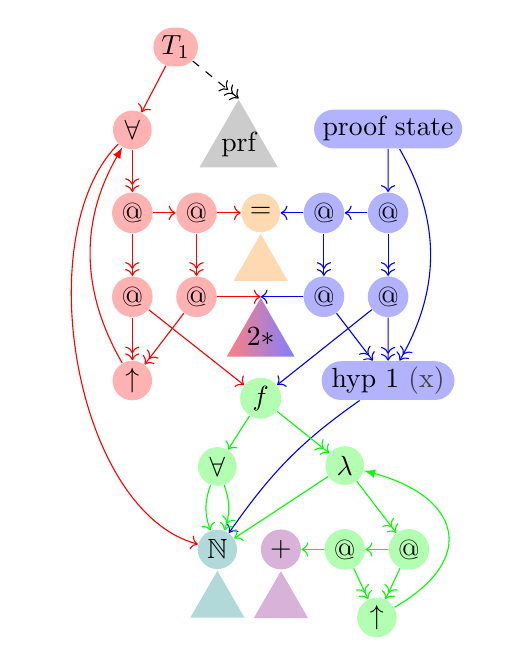
\begin{tikzpicture}[
  lnode/.style = {fill=gray!40, circle, inner sep = 1.5, minimum height=14, },
  nred/.style = {fill=red!30},
  nblue/.style = {fill=blue!30},
  ngreen/.style = {fill=green!30},
  npurple/.style = {fill=teal!30},
  nyellow/.style = {fill=violet!30},
  norange/.style = {fill=orange!30},
  mred/.style = {draw=red},
  mblue/.style = {draw=blue},
  mgreen/.style = {draw=green},
  mpurple/.style = {draw=pink},
  myellow/.style = {draw=violet},
  morange/.style = {draw=orange},
  ]
  \node[lnode, nred] (forall1) at (0, 0) {$\forall$};
  \node[lnode, nred, below = 0.8 of forall1, anchor=center] (app1) {@};
  \node[lnode, nred, right = 0.55 of app1, anchor=center] (app2) {@};
  \node[lnode, norange, right = 0.55 of app2, anchor=center] (eq) {$=$};
  \node[lnode, norange, regular polygon, regular polygon sides=3, inner sep = 4,
  below = 0 of eq, anchor = north] (eqt) {};
  \node[lnode, nred, below = 0.8 of app2, anchor=center] (app3) {@};
  \node[lnode, fill=white, regular polygon, regular polygon sides=3, inner sep = 0,
  right = 0.55 of app3, anchor = north,
  shade, left color=red!50, right color=blue!50] (2times1) {$2*$};
  \node[lnode, nred, below = 0.8 of app1, anchor=center] (app6) {@};
  \node[lnode, nblue, right = 0.55 of eq, anchor=center] (app7) {@};
  \node[lnode, nblue, below = 0.8 of app7, anchor=center] (app12) {@};
  \node[lnode, nblue, right = 0.55 of app7, anchor=center] (app11) {@};
  \node[lnode, nblue, below = 0.8 of app11, anchor=center] (app8) {@};
  \node[lnode, ngreen, below = 2.1 of eq, anchor=center] (f) {$f$};
  \node[lnode, nred, below left = 0.8 and 0 of app6.south, anchor=center] (v1) {$\uparrow$};
  \node[lnode, nblue, rounded rectangle, below right = 0.8 and 0 of app8.south, anchor=center] (hyp1) {hyp 1 \color{darkgray}(x)};
  \node[lnode, nblue, rounded rectangle, above = 0.8 of app11, anchor=center] (ps) {proof state};
  \node[lnode, ngreen, below left = 0.6 and 0.55 of f.south, anchor=center] (forall2) {$\forall$};
  \node[lnode, npurple, below = 0.8 of forall2, anchor=center] (nat) {$\mathbb{N}$};
  \node[lnode, npurple, regular polygon, regular polygon sides=3, inner sep = 4,
  below = 0 of nat, anchor = north] (natt) {};
  \node[lnode, nyellow, right = 0.55 of nat, anchor=center] (plus) {$+$};
  \node[lnode, nyellow, regular polygon, regular polygon sides=3, inner sep = 4,
  below = 0 of plus, anchor = north] (plust) {};
  \node[lnode, ngreen, right = 0.55 of plus, anchor=center] (app9) {@};
  \node[lnode, ngreen, right = 0.55 of app9, anchor=center] (app10) {@};
  \node[lnode, ngreen, above = 0.8 of app9, anchor=center] (lambda1) {$\lambda$};
  \node[lnode, ngreen, below = 0.6 of $(app9.south)!0.5!(app10.south)$, anchor=center] (v2) {$\uparrow$};
  \node[lnode, nred, rounded rectangle, above right = 0.8 and 0.55 of forall1.north, anchor=center] (T1) {$T_1$};
  \node[lnode, regular polygon, regular polygon sides=3, inner sep = -0.5,
  below right = 0.4 and 0.8 of T1.south, anchor = north] (proof) {prf};

  \draw[->>, mred] (forall1) -- (app1);
  \draw[->, mred] (app1) -- (app2);
  \draw[->, mred] (app2) -- (eq);
  \draw[->>, mred] (app2) -- (app3);
  \draw[->, mred] (app3) -- (2times1.north);
  \draw[->>, mred] (app3) -- (v1);
  \draw[->>, mred] (app1) -- (app6);
  \draw[->>, mred] (app6) -- (v1);
  \draw[-latex, mred] (v1) to[out=120, in=-120] (forall1);
  \draw[->, mred] (forall1) to[out=-135, in=165, looseness=0.8] (nat);
  \draw[->, mred] (T1) -- (forall1);
  \draw[->, mred] (app6) -- (f);
  \draw[->>, mblue] (app11) -- (app8);
  \draw[->, mblue] (app8) -- (f);
  \draw[->>, mblue] (app8) -- (hyp1);
  \draw[->, mblue] (app7) -- (eq);
  \draw[->, mblue] (ps) -- (app11);
  \draw[->, mblue] (app11) -- (app7);
  \draw[->>, mblue] (app7) -- (app12);
  \draw[->, mblue] (app12) -- (2times1.north);
  \draw[->>, mblue] (app12) -- (hyp1);
  \draw[->>, mblue] (ps) to[out=-60, in=60] (hyp1);
  \draw[->, mblue] (hyp1) to[out=-145, in=55] (nat);
  \draw[->, mgreen] (f) -- (forall2);
  \draw[->>, mgreen] (f) -- (lambda1);
  \draw[->, mgreen] (forall2) to[out=-110, in=110] (nat);
  \draw[->>, mgreen] (forall2) to[out=-70, in=70] (nat);
  \draw[->, mgreen] (lambda1) -- (nat);
  \draw[->>, mgreen] (lambda1) -- (app10);
  \draw[->, mgreen] (app10) -- (app9);
  \draw[->, mgreen] (app9) -- (plus);
  \draw[->>, mgreen] (app9) -- (v2);
  \draw[->>, mgreen] (app10) -- (v2);
  \draw[-latex, mgreen] (v2) to[out=30, in=-15, looseness=1.8] (lambda1);
  \draw[->>>, dashed] (T1) -- (proof.north);
\end{tikzpicture}
\end{minipage}

\end{document}
% Local Variables:
% TeX-command-extra-options: "-shell-escape"
% End: